\documentclass[10pt,twocolumn,letterpaper]{article}

\usepackage{cvpr}
\usepackage{times}
\usepackage{epsfig}
\usepackage{graphicx}
\usepackage{amsmath}
\usepackage{amssymb}

\usepackage{color}
\usepackage{mathtools}
\usepackage{mathptmx}
\usepackage[11pt]{moresize}
\usepackage{wrapfig}
\usepackage{bbm}
\usepackage{xcolor}
\usepackage{tabularx}
\usepackage{bm}



\newcommand{\R}{\mathbb{R}}
\newcommand{\E}{\mathbb{E}}
\newcommand{\N}{\mathbb{N}}
\newcommand{\Z}{\mathbb{Z}}
\newcommand{\V}{\mathbb{V}}
\newcommand{\Q}{\mathbb{Q}}
\newcommand{\K}{\mathbb{K}}
\newcommand{\C}{\mathbb{C}}
\newcommand{\T}{\mathbb{T}}
\newcommand{\I}{\mathbb{I}}

% Include other packages here, before hyperref.

% If you comment hyperref and then uncomment it, you should delete
% egpaper.aux before re-running latex.  (Or just hit 'q' on the first latex
% run, let it finish, and you should be clear).
\usepackage[breaklinks=true,bookmarks=false]{hyperref}

\cvprfinalcopy % *** Uncomment this line for the final submission

\def\cvprPaperID{****} % *** Enter the CVPR Paper ID here
\def\httilde{\mbox{\tt\raisebox{-.5ex}{\symbol{126}}}}

% Pages are numbered in submission mode, and unnumbered in camera-ready
%\ifcvprfinal\pagestyle{empty}\fi
\setcounter{page}{1}
\begin{document}

%%%%%%%%% TITLE
\title{ Probabilistic Wind Power Forecasting using Stochastic Differential Equations }  % \\  \small{Report}}

\author{ Waleed Alhaddad\textsuperscript{\textasteriskcentered} \qquad Ra\'ul  Tempone\textsuperscript{\textasteriskcentered}\textsuperscript{\textdagger} \\
\textsuperscript{\textasteriskcentered}CEMSE Division, King Abdullah University of Science and Technology (KAUST), Saudi Arabia \\ \textsuperscript{\textdagger}Alexander von Humboldt Professor in Mathematics of Uncertainty Quantification\\ RWTH Aachen University,  Germany
}

\maketitle
%\thispagestyle{empty}

%%%%%%%%% ABSTRACT

\begin{abstract}
Reliable wind power generation forecasting is crucial to meeting energy demand through renewable power sources, to trade excess power and to the design of investment strategies. We propose a parametric forecast error model to a model to simulate forecast error and quantify its uncertainty. It also provide a basis to calibrate a forecast model for  optimal dispatch of electric power. This model is based on parametric Stochastic Differential Equations (SDE's) and an approximate Maximum Likelihood method based on continuous optimization.The result is a skewed stochastic process that simulates the uncertainty of wind power forecasts accounting for maximum power production limit and other temporal effects. We apply the model to historical Uruguayan data and forecasts (2016-2017).



\end{abstract}

%%%%%%%%% BODY TEXT
\section{Introduction}
	Wind power forecasting is complex to model and inherits a lot of uncertainty. The link between physical models of  wind turbines  and power production is non-trivial, non-linear and sensitive to the configuration and state of the wind farm. Reliable wind power forecasting is essential and can provided by probabilistic forecasts.

	There are many possible techniques to prepare probabilistic forecasts.  In this work, we focus on the use of Stochastic Differential Equations (SDE's) to represent and quantify uncertainties in wind power forecasts. It is important to note that this approach is  forecast technology agnostic. Moreover, it can be used to calibrate and integrate wind power forecasts into optimal electrical power dispatch models. Also, it could serve as a basis for assessments of wind power forecasts  and uncovering their particularities.

Previous attempt by M\o ller et al. (M\o ller, Zugno, \& Madsen, 2016)  considered probabilistic wind power forecast models based on SDE's. Here, we propose an improved model featuring derivative tracking and  non-Gaussian skew symmetric approximations of the stochastic process both of which are essential in wind power probabilistic forecasting. We apply the model to Uruguayan wind power forecasts together with Uruguayan historical data  pertaining to the year 2016-2017.

%-------------------------------------------------------------------------
\section{Phenomenological  Model}

Let $X_t$ be the  wind power generation forecasts stochastic process defined by the  following parameterized stochastic differential equation (SDE),
\begin{equation}
\begin{split}
dX_t &= a(X_t; \bm{\theta}) dt + b (X_t; \bm{\theta} ) dW_t \quad t > 0 \\
X_0 & = X_0
\end{split}
\label{main}
\end{equation}

\begin{itemize}
%\item $\Delta_N$: any function of the number of samples, $N$. For example, $\Delta_N = \frac{1}{N}$.
\item $a(\cdot; \bm{\theta}):[0,1] \to \R $  a drift function.
\item $b (\cdot; \bm{\theta} ):[0,1] \to \R$  a  diffusion function.
\item $\bm{\theta}$: a vector of parameters.
\item $W_t$: Standard Wiener random process in $\R$.
\end{itemize}



\subsection{Physical Constrains}

Let $p_t$ be a numerical wind power forecast, which is an input to this approach. Then the model is given by the following It\^{o} stochastic differential equation,
\begin{equation}
\begin{split}
dX_t&= \dot{p} \ dt + (\theta_t -X_t) \ dt + b (X_t; \bm{\theta} ) \ dW_t \quad t > 0 \\
X_0&=x_0
\end{split}
\end{equation}
Note that the process $X_t$ mean reverts to  the wind power forecast $p_t$ and  tracks its the time derivative $\dot{p}_t$.  An example such mean reverting model without derivative tracking exhibits consistent lags as shown in Figure (\ref{sine_wave_shift}).

As the  installed power production capacity is limited, we normalize with respect to the installation power. Thus our process must be limited to the range $[0,1]$. To enforce this constraint, we must have drift and diffusion control.
\subsubsection*{Diffusion Control: } The physical constraint is respected  by choosing  diffusion coefficient $ b (x; \bm{\theta} )= \sqrt{2 \theta_t \alpha p_t(1-p_t) x (1-x)} $ that is zero on the boundaries of $[0,1]$. Note that $\alpha$ is a path variability constant parameter to be determined.
\subsubsection*{Drift Control: }

Observe that the term $\dot{p}_t $ is not controlled to maintain that $X_t$ stays a.s.  inside the range $[0,1]$. In other words, the zero drift line defined by $a(X_t; \bm{\theta}) =0$ must  be contained inside the range $[0,1]$. Thus, must have that,
\begin{equation}
\frac{- |\dot{p_t}|}{p_t} \leq \theta \leq \frac{|\dot{p}_t|}{1- p_t}
\end{equation}

which is satisfied  by choosing $\theta_t$ as follows,
\begin{equation}
\theta_t = \max \left( \theta_0 \ , \ \frac{|\dot{p}_t|}{\min (p_t, 1-p_t)}  \right ) \label{theta_t}
\end{equation}

\subsubsection*{Change of Variables:}
In order to avoid differentiation of the forecast $\dot{p}_t$ and simplify, we apply a change of variables $$V_t = X_t - p_t$$  \\
The  model becomes,
\begin{equation}
\begin{split}
dV_t &=  - \theta_t V_t \  dt + \sqrt{2 \theta_t \alpha p_t(1-p_t) (V_t +p_t ) (1-V_t-p_t)} \  dW_t  \\ %\quad t > 0
V_0 & = v_0
\end{split}\label{main}
\end{equation}
with $\theta_t$ given by (\ref{theta_t}).







%%%%%%%%%%%%%%%%%%%%%%%%%%%%%%%%%%%%%%%%



However, this does not track the rate of change of the forecast $\dot{p}$ which  results in $X_t$ being out of sync with the forecast  as can be seen in Figure (\ref{sine_wave_shift})

\begin{figure}[t]
\begin{center}
%\fbox{\rule{0pt}{2in} \rule{0.9\linewidth}{0pt}}
   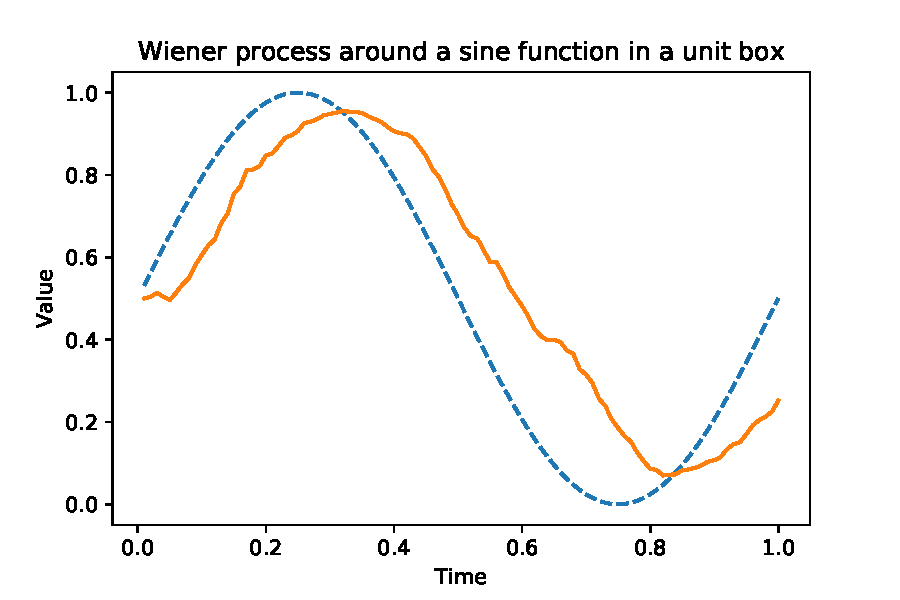
\includegraphics[width=0.8\linewidth]{conv_sine_shift.pdf}
\end{center}
   \caption{Example of the process $X_t$ following a sine wave without derivative tracking.}
\label{fig:long}
\label{fig:onecol}
\label{sine_wave_shift}
\end{figure}


%%%%%%%%%%%%%%%%%%%%%%
\section{Data}

We apply the model to Uruguayan wind power generation data and their corresponding numerical wind power production forecast.The wind power generation data set contains hourly samples of aggregated wind power production throughout the country. Each sample path contains 72 hourly observations and we have a total of 1217 sample paths spanning the year 2016 to 2017 (87,624 data points). The numerical wind power generation forecast set contains  1217 forecasts of the wind power generation  corresponding to the actual  wind power generation data set mentioned above.

\begin{figure}[t]
\begin{center}
%\fbox{\rule{0pt}{2in} \rule{0.9\linewidth}{0pt}}
   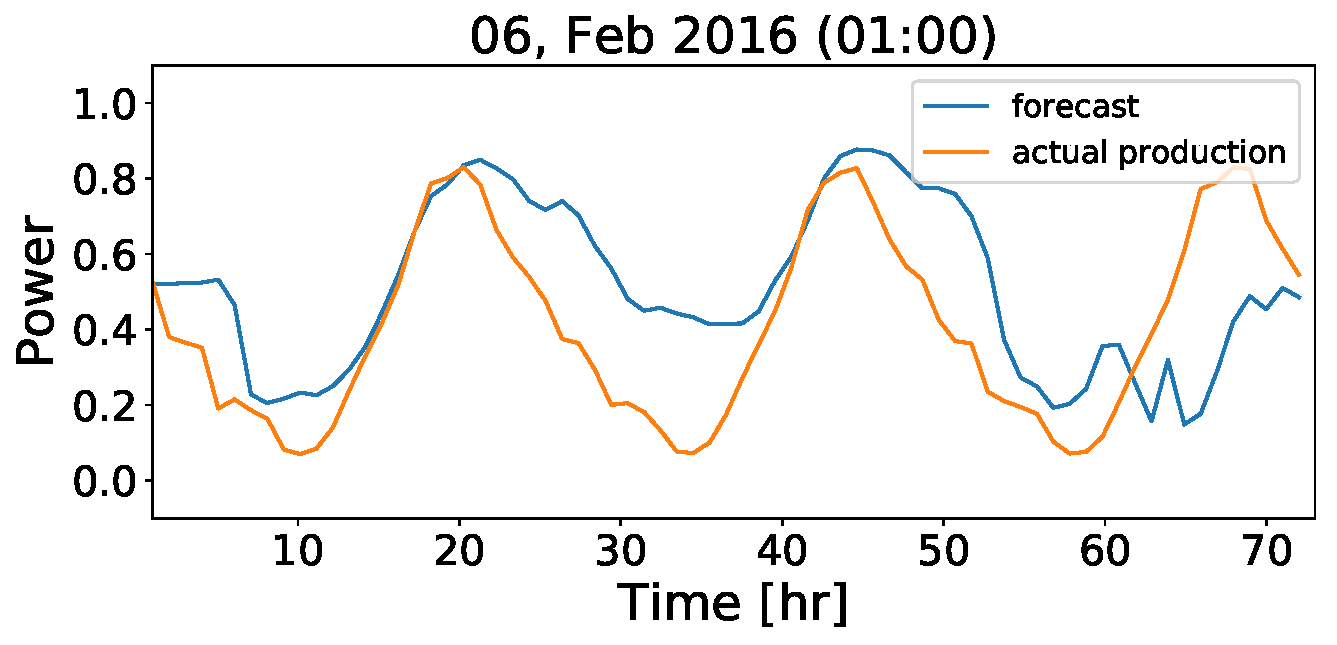
\includegraphics[width=0.8\linewidth]{Forecast_data_68.pdf}
    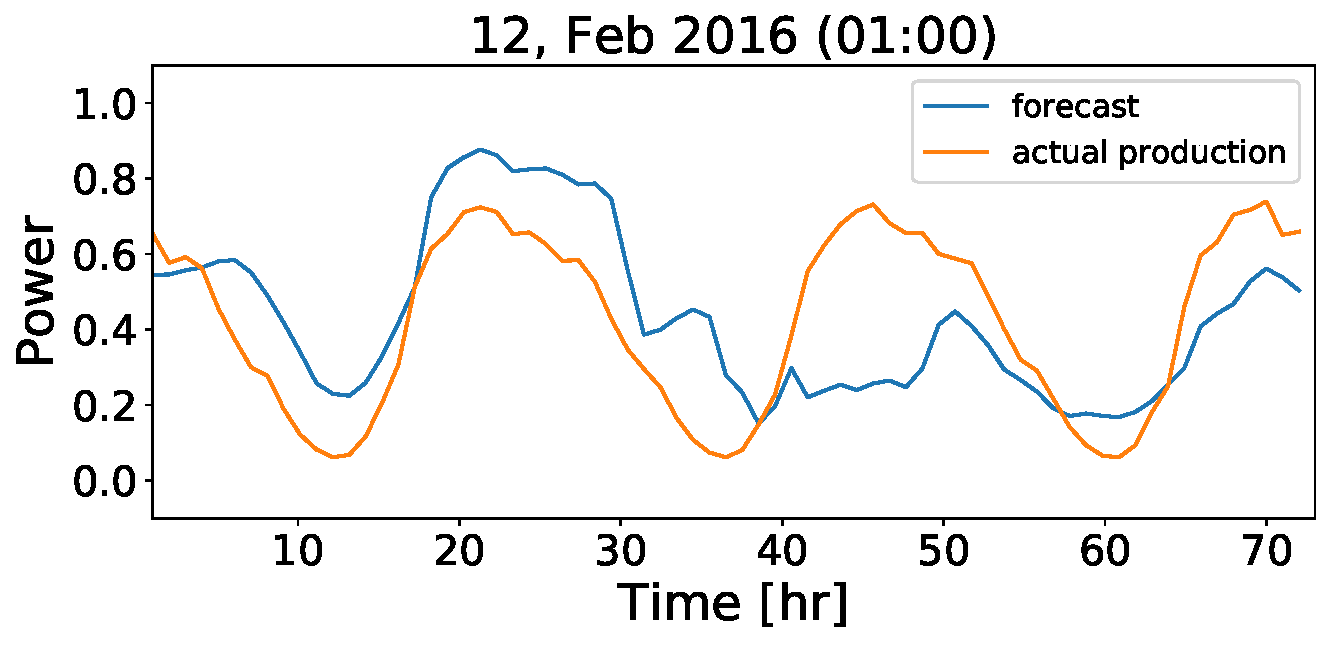
\includegraphics[width=0.8\linewidth]{Forecast_data_82.pdf}
\end{center}
   \caption{Examples of wind power generation from the data set along with the wind power generation forecast.}
\label{fig:long}
\label{fig:onecol}
\end{figure}

\section{Inference and Optimization}

\subsection{Likelihood}
The SDE above defines the stochastic process $V_t$. Consider a set of M paths with N observations each, $ V^{M,N}=\{ V_{t_1^{M,N}} , V_{t_2^{M,N}} ,\ldots , V_{t_N^{M,N}} \}$ observed in intervals of $\Delta_N$. Since $V_t$ is Markovian, the likelihood function is given by  product of its  transition densities.

\begin{equation}
\mathcal{L}(\bm{\theta};V) =\prod\limits_{j=1}^M \prod\limits_{i=1}^N \rho ( {V_{j,i+1}|V_{j,i}}, \bm{\theta})  \rho (V_{j,0})
\label{likelihood}
\end{equation}

\subsection{Approximate Likelihood}
Solving for transition densities of the process $V_t$ requires solving the Fokker-Planck equation at every step which is computationally prohibitive. A common choice is performing a  Gaussian approximation of the transition densities, but this is inappropriate here due to physical constraints. \\

Therefore, we propose an approximate likelihood inspired by the stationary distribution of the process $X_t$ which is a Beta distribution for a constant forecast $p_t$.Additionally,  as the process $X_t$ and $p_t$ take on values in $[0,1]$, then $V_t$ takes on values in $[-1,1]$. Therefore,  it is natural to use a  Beta distribution with compact support on $[-1,1]$.

%We obtain the modified Beta distribution,
%
%\begin{equation}
%\begin{split}
%f_Y(y; \alpha , \beta )&= f_X(g^{-1}(y) ) \Big| \frac{\partial g^{-1}(y)}{\partial y }  \Big| \\
%&= \frac{1}{B(\alpha, \beta) (b-a)} \Big(\frac{a-y}{b-a}\Big)^{\alpha -1}\Big(1-\frac{a-y}{b-a} \Big)^{\beta -1} \label{modified_Beta}
%\end{split}
%\end{equation}
%where $B(\cdot,\cdot)$ is the Beta function. Also, we have that
%\begin{equation}
%\E[Y]= a + (b-a) \frac{\alpha}{\alpha + \beta}
%\end{equation}
%\begin{equation}
%\V[Y]= (b-a)^2 \frac{\alpha \beta}{(\alpha + \beta)^2 (\alpha + \beta + 1)}
%\end{equation}

\subsubsection*{ Moment Matching}
To approximate the transition densities of  the process $V_t$, we match its moments with the shape parameters $\xi_1, \xi_2$ of the Beta distribution on $[-1,1]$.  Then, the shape parameters are given by,
\begin{equation}
\xi_1 = - \frac{(1+\tilde{\mu}_t )(\tilde{\mu}_t^2 + \tilde{\sigma}_t^2 -1)}{2 \tilde{\sigma}_t^2} \quad \xi_2=  \frac{(\tilde{\mu}_t-1 )(\tilde{\mu}_t^2 + \tilde{\sigma}_t^2 -1)}{2 \tilde{\sigma}_t^2} \label{param_transformed_beta}
\end{equation}
where $\tilde{\mu}_t = m_1(t)$ and $\tilde{\sigma}_t^2= m_2(t)- m_1^2(t)$ and $m_i$ being the i-th moment of the process $V_t$. Using It\^{o}'s formula, the first two moments  of the  process $V_t$ are given by,
\begin{equation}
\begin{split}
 \frac{dm_1(t_n)}{dt} &=    - \theta_t m_1(t_n)  \\
\frac{d m_{2}(t_n)}{dt}&= -2m_{2}(t_n) [\theta_t + \alpha \theta_t p_t(1-p_t) ] \\
&+ 2m_{1}(t_n)[\alpha \theta_t p_t (1-p_t) (1-2p_t)] \\
&+ 2\alpha \theta_t p_t^2(1-p_t)^2  \\
%m_2(0) = \E[V_0^2] = v_0^2\\
\end{split}
\end{equation}
with initial conditions, $m_1(t_{n-1})= v_{n-1}$ and $m_2(t_{n-1})= v_{n-1}^2$.
\subsection{Optimization}
Let $\ell$ be the natural logarithm  of the likelihood in $(\ref{likelihood})$. Given the data set $V^{M,N}$, we  optimize the the log-likelihood $\ell$  using L-BFGS algorithm  for the optimal parameters $\theta_0^* , \alpha^*$ as follows,
\begin{equation}
(\theta_0^* , \alpha^* ) = \arg \underset{\theta_0, \alpha>0}{\min} - \ell( \theta_0,  \alpha | V^{M,N} )
\end{equation}
The contours of the  log-likelihood can be seen in Figure (\ref{contour}).To further inspect the log-likelihood at the point of optimality $(\theta_0^* , \alpha^* )$, we look at the ellipse defined by the  Hessian of the log-likelihood at the point of optimality.  We observe that the ellipse shrinks at a fast rate as shown in Figure (\ref{ellipse_drawing}). We see that  the convergence rate of the parameters $\theta_0$ and $\alpha$ is slightly faster than the expected rate of $1/\sqrt{M}$. This is due to the correlation structure of the process $V_t$, thus a path may act  as more than one  uncorrelated sample. We note that the uncertainty in determining the parameter $\alpha$  is much higher than  in $\theta_0$.

\begin{figure}[t]
\begin{center}
%\fbox{\rule{0pt}{2in} \rule{0.9\linewidth}{0pt}}
   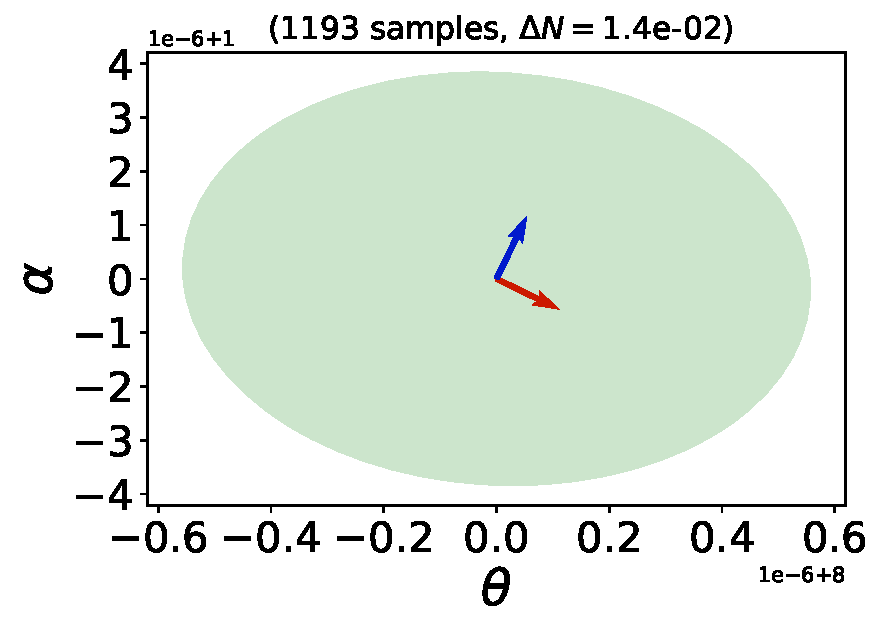
\includegraphics[width=0.6\linewidth]{ellipse1193_samples_dN=14e-02.pdf}
    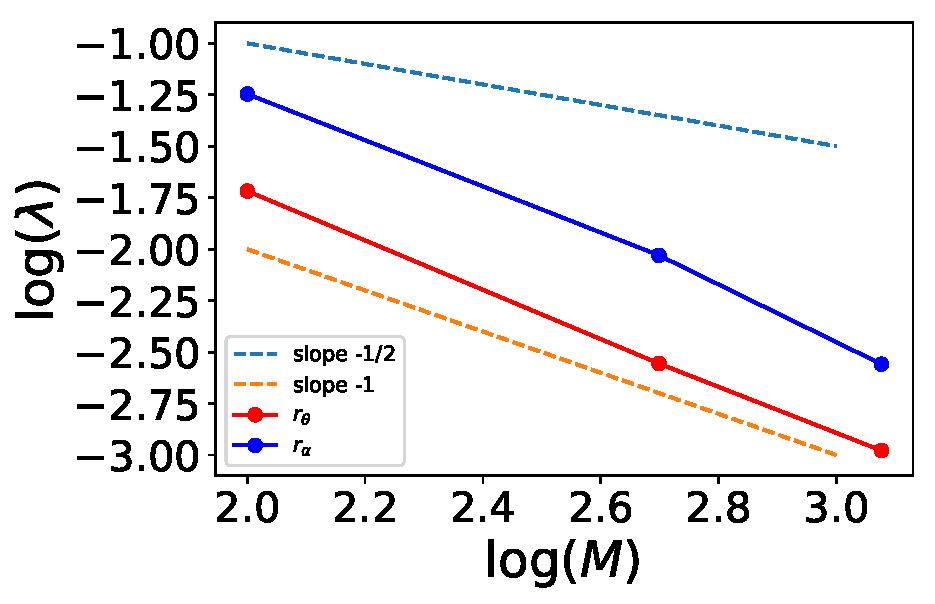
\includegraphics[width=0.6\linewidth]{ellipse_conv_samples_dN=14e-02.pdf}
\end{center}
   \caption{Left:Shrinkage of the ellipse determined by the Hessian matrix of the log-likelihood around the point of optimality $(\theta_0^*, \alpha^*)\approx (8,1)$ (Axis are not in natural scale, arrows only to  eignevector direction). Right: Convergence of the major and semi-axis of the ellipse  of the Hessian of the log-likelihood at the point optimality $(\theta_0^*, \alpha^*)\approx (8,1)$. Note that it is slightly faster than the expected rate of $1/\sqrt{M}$. This is due to the correlation structure of the process $V_t$, thus a path may act  as more than one  uncorrelated sample.}
\label{ellipse_drawing}
\end{figure}

 \begin{figure}[t]
\begin{center}
%\fbox{\rule{0pt}{2in} \rule{0.9\linewidth}{0pt}}
   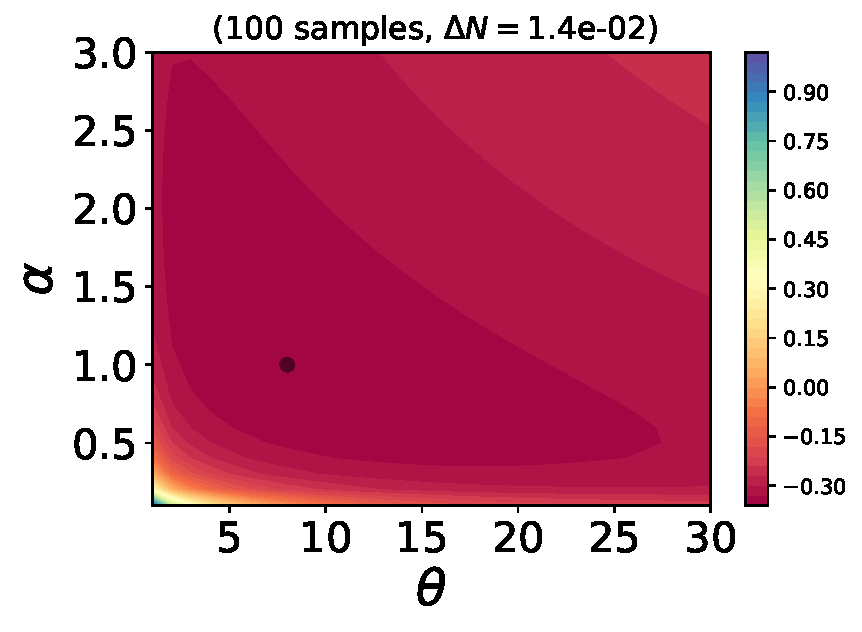
\includegraphics[width=0.9\linewidth]{ISO_100_samples_dN=14e-02.pdf}
   %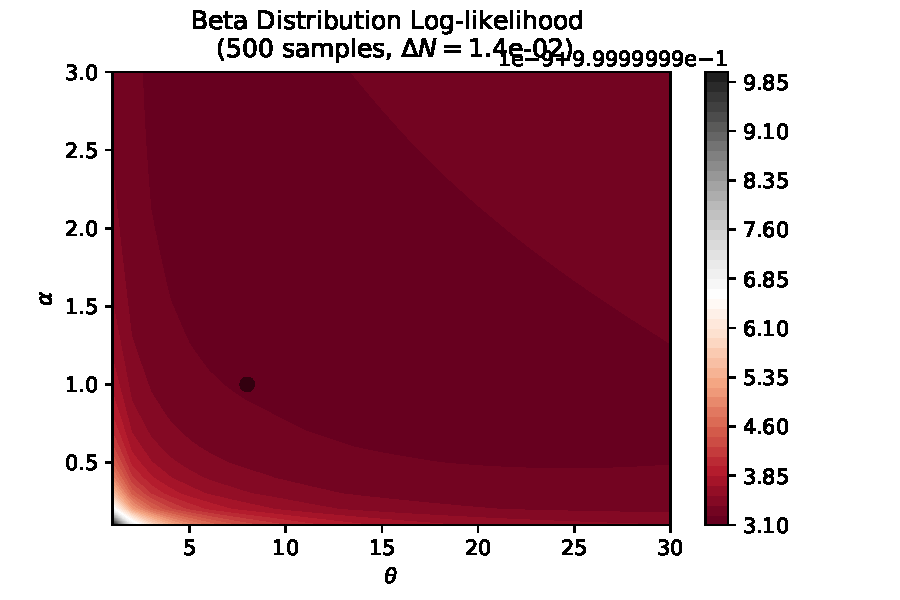
\includegraphics[width=0.5\linewidth]{ISO_500_samples_dN=14e-02.pdf}
   %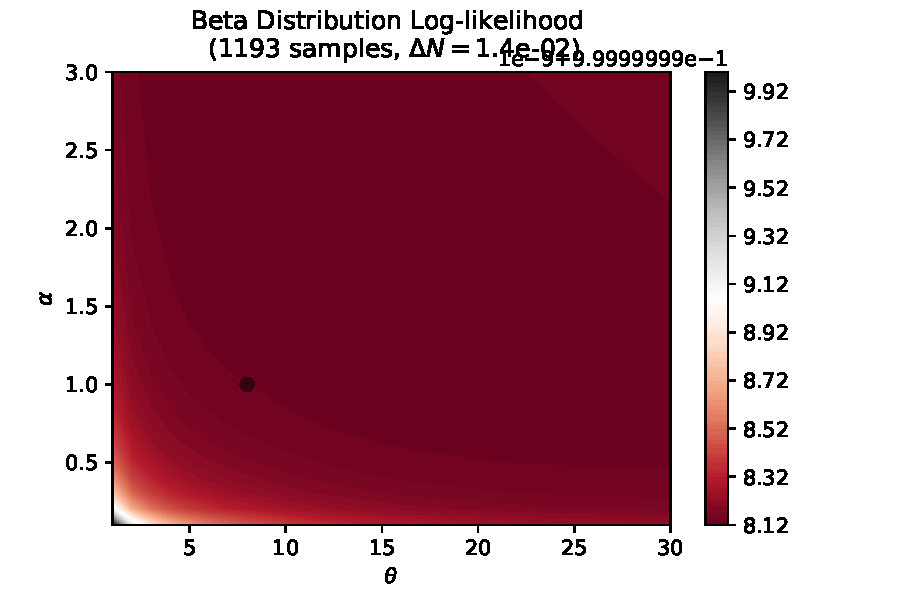
\includegraphics[width=0.5\linewidth]{ISO_1193_samples_dN=14e-02.pdf}
\end{center}
   \caption{Contour plot of the log-likelihood with only 100 sample paths, point of optimality $(\theta_0^*, \alpha^*)\approx (8,1)$ indicated by the  black dot.}
\label{contour}
\end{figure}







%%%%%%%%%%%%%%%%%%%%%%


\section{Results}
 We are able to obtain the parameters based on the complete data sets mentioned earlier. The parameters are given by $(\theta^*, \alpha^*)\approx (8,1)$.


%We can also see in Figure() that the region surrounding the optimal parameters becomes more defined as we add more sample paths.

In Figure (\ref{fig:72hr}) and (\ref{fig:6hr}), we simulate sample forecast errors $V_t$ using the optimal parameters  $(\theta_0^*, \alpha^*)\approx (8,1)$ and obtain the associated confidence bands empirically using 1000 sample paths of each forecast. %Note that the confidence bands obtained are non-trivial and reflect the complexity of the uncertainties in numerical wind power generation forecasts.

\begin{figure}[t]
\begin{center}
%\fbox{\rule{0pt}{2in} \rule{0.9\linewidth}{0pt}}
   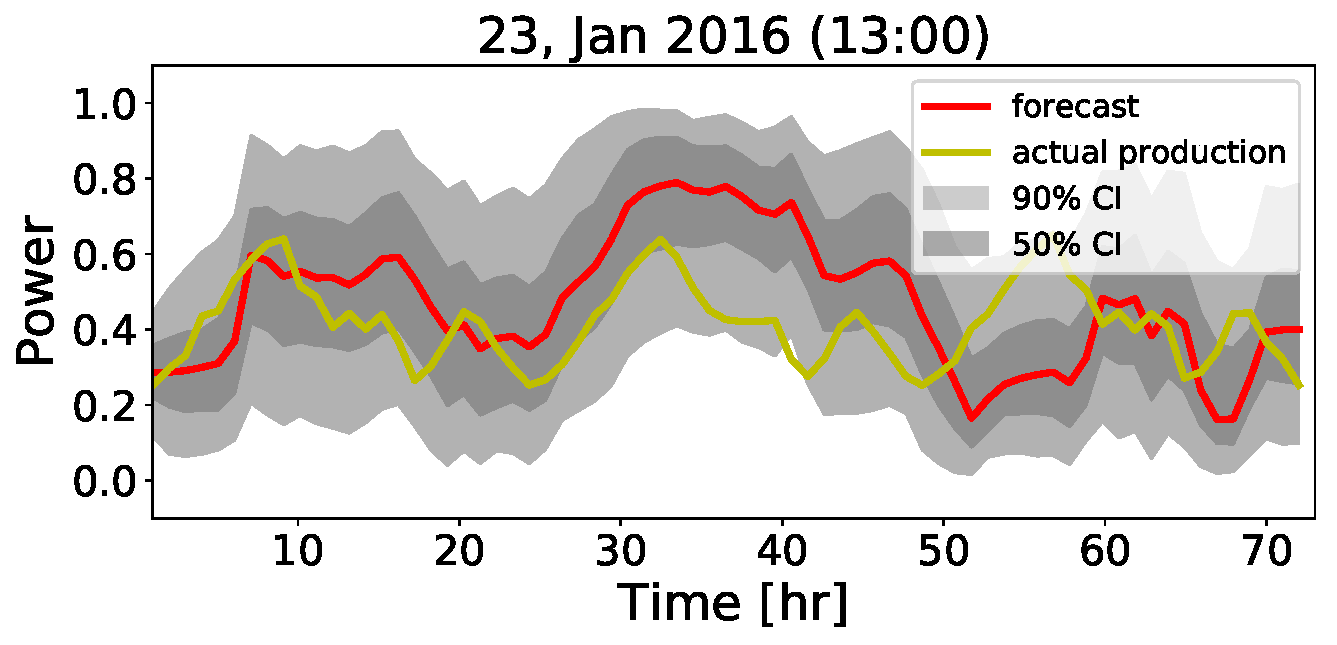
\includegraphics[width=0.8\linewidth]{72hr_forecast_CI_31.pdf} %667
   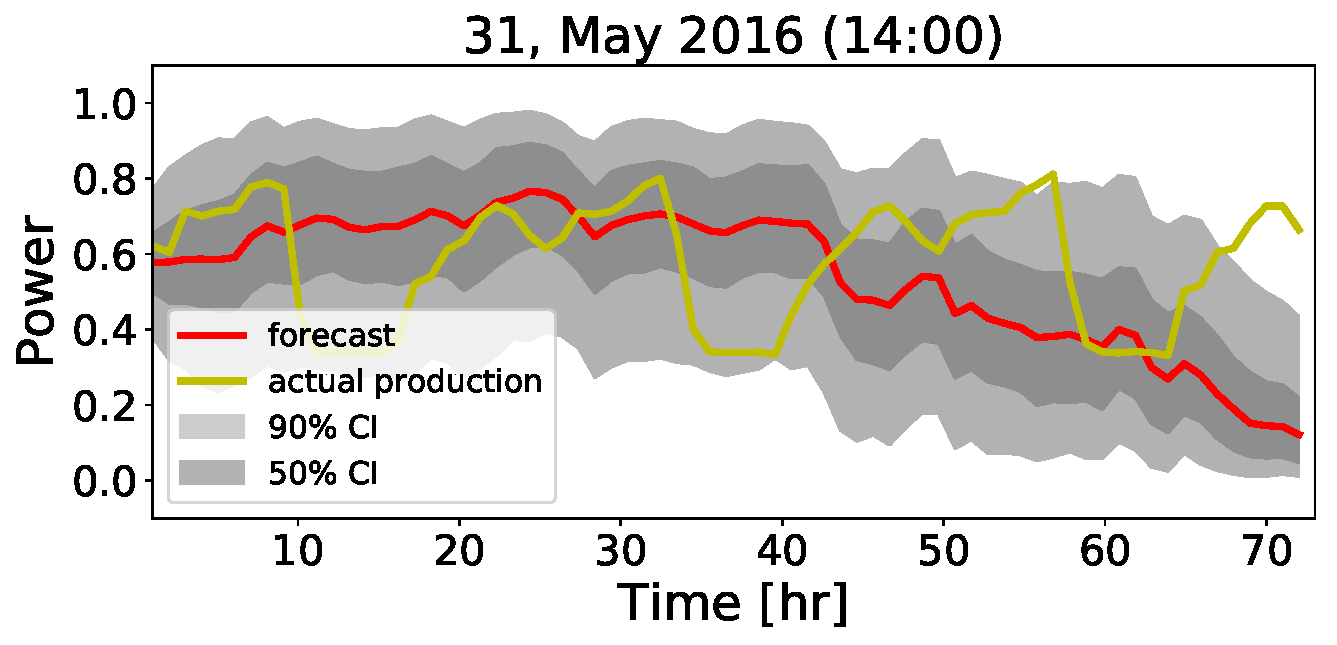
\includegraphics[width=0.8\linewidth]{72hr_forecast_CI_437.pdf}
   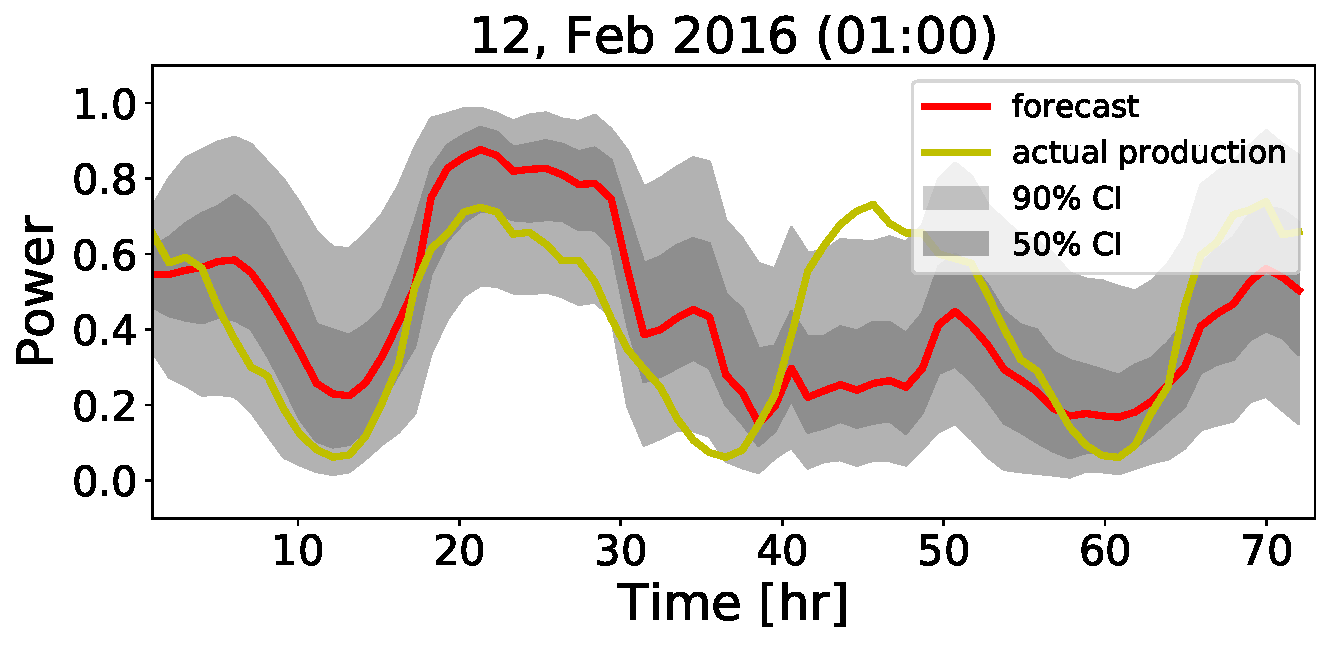
\includegraphics[width=0.8\linewidth]{72hr_forecast_CI_82.pdf}

\end{center}
   \caption{ Examples of confidence bands obtained for the full 72 hour forecasts.We can see that the model captures the fluctuations in the actual production with non-trivial and asymmetric confidence intervals.}
\label{fig:72hr}
\end{figure}

\begin{figure}[t]
\begin{center}
%\fbox{\rule{0pt}{2in} \rule{0.9\linewidth}{0pt}}
   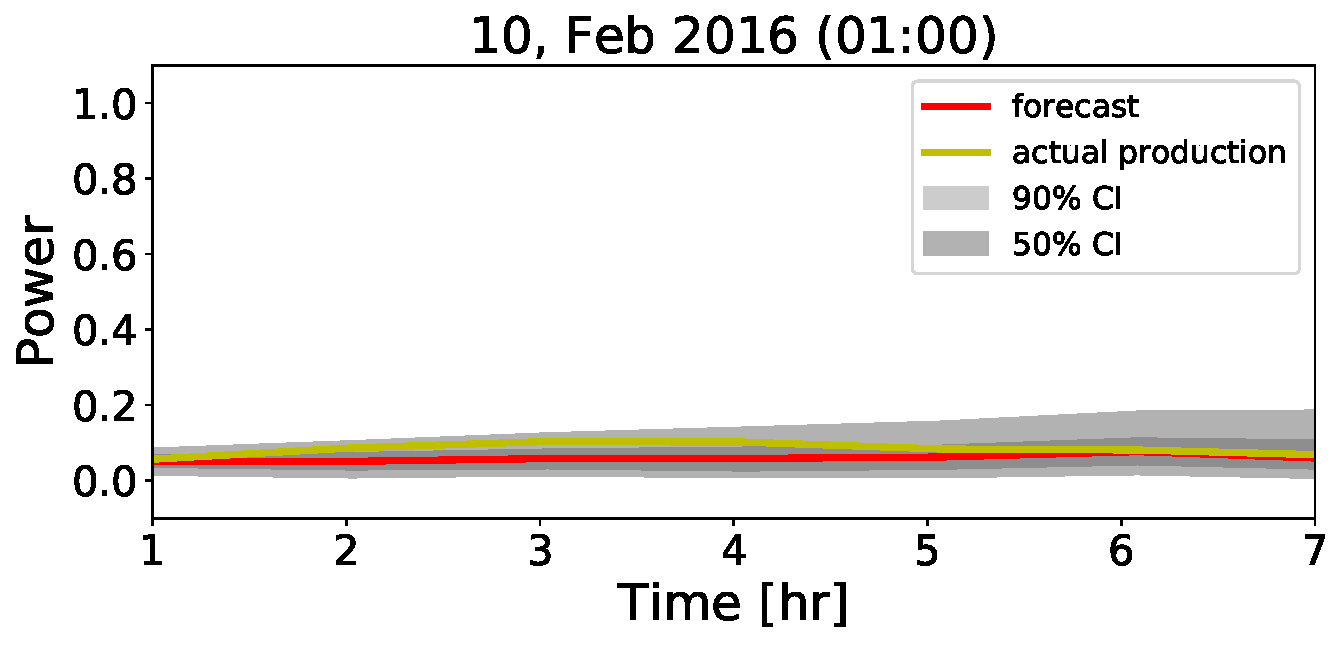
\includegraphics[width=0.8\linewidth]{6hr_forecast_CI_75.pdf}  %569
   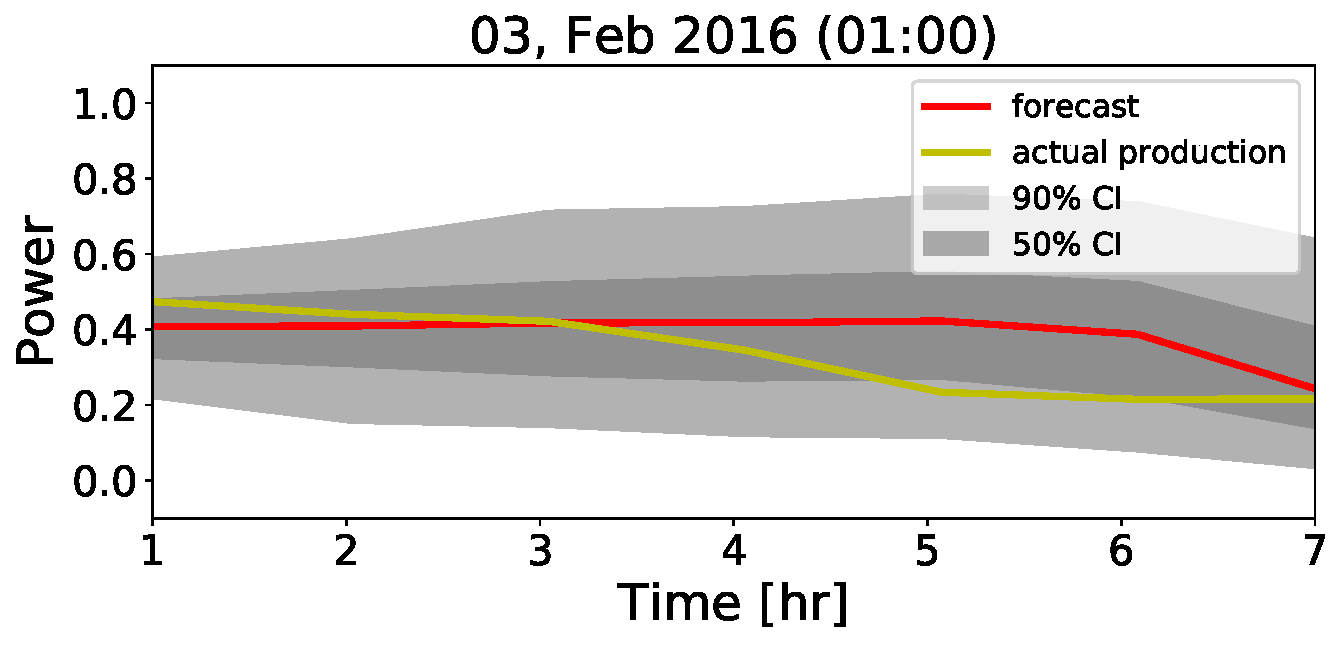
\includegraphics[width=0.8\linewidth]{6hr_forecast_CI_59.pdf}
   %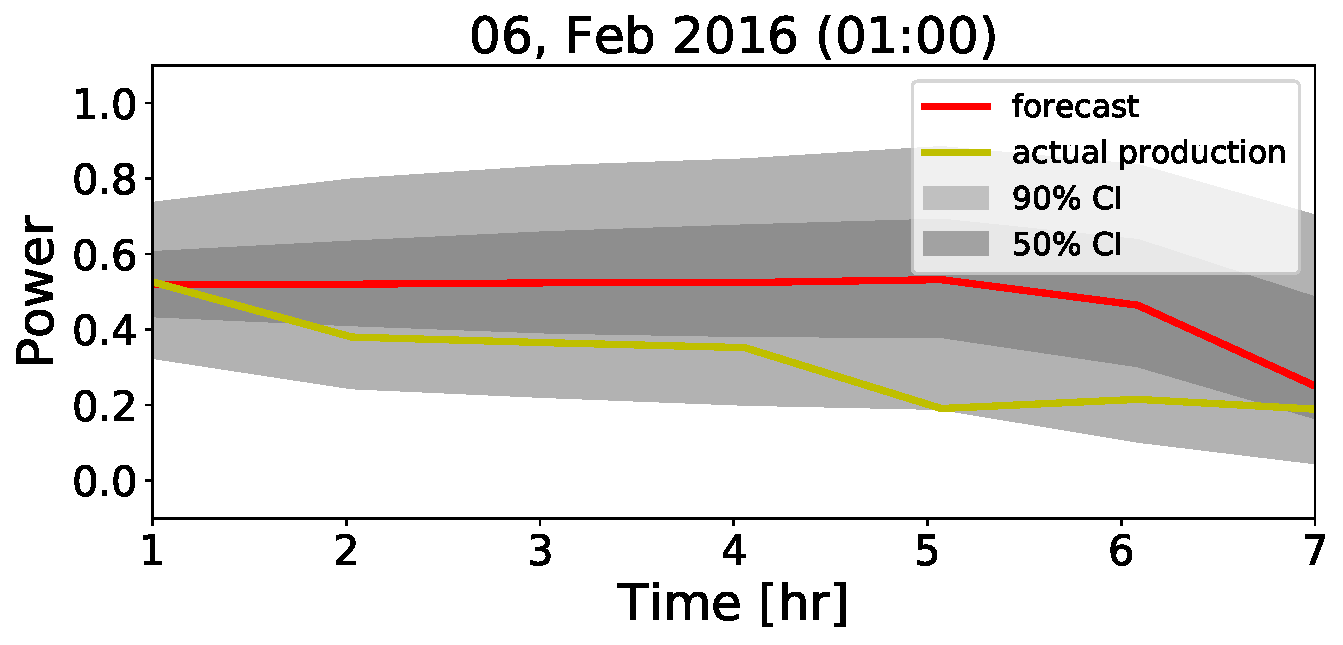
\includegraphics[width=0.9\linewidth]{6hr_forecast_CI_68.pdf}
\end{center}
   \caption{ Examples of confidence bands obtained for the first 6 hours of the forecasts. This is important as this specific forecasting company computes a new forecast every 6 hours for reliability.}
\label{fig:6hr}
\end{figure}


 \begin{figure}[t]
\begin{center}
%\fbox{\rule{0pt}{2in} \rule{0.9\linewidth}{0pt}}
   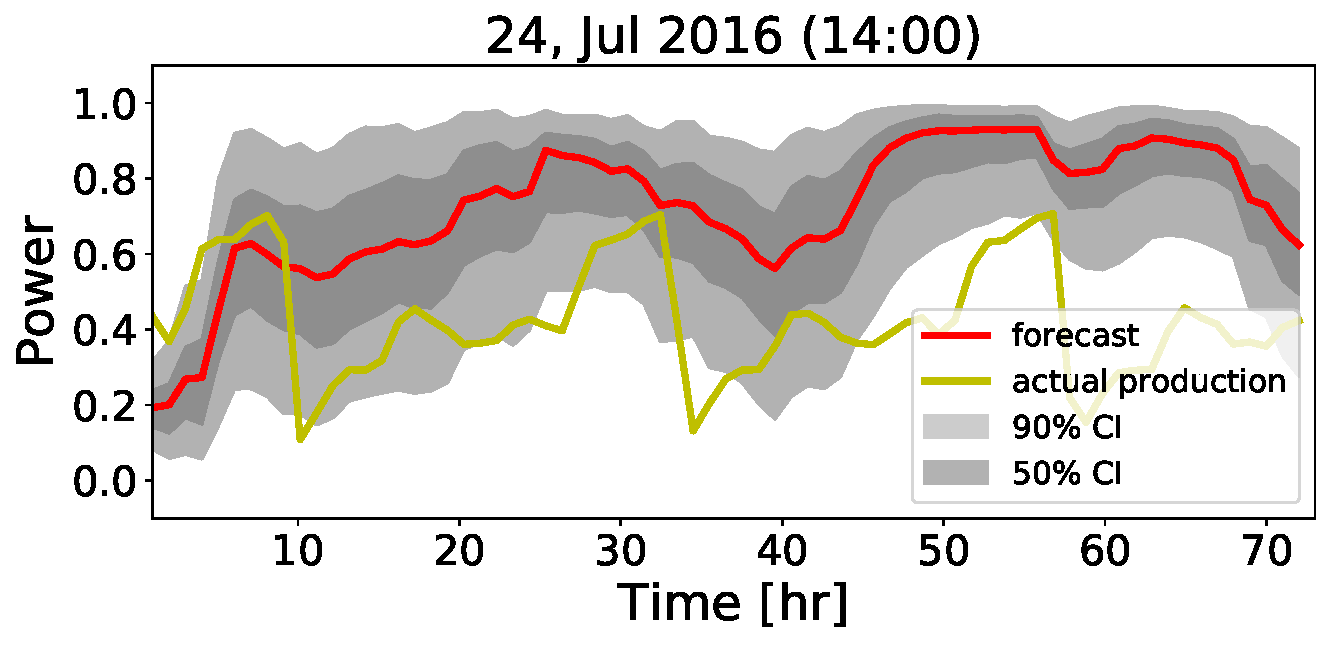
\includegraphics[width=0.8\linewidth]{72hr_forecast_CI_623.pdf}  %569
\end{center}
   \caption{ Examples of omitted data which corresponds to production control and manual energy management decisions. In this example,  wind power production was repeatedly curtailed at around 2 AM which is a period of low power demand. Automatic detection of such scenarios is to be incorporated in future works.}
\label{fig:6hr}
\end{figure}

\section{Conclusions}
We have proposed a model based on SDE's to quantify uncertainties in wind power generation forecasts. A parametric SDE to represent and quantify  uncertainty in wind power forecasts. It is forecast technology agnostic. Moreover, it provides a basis for decision making in the optimal dispatch of electric power.


%\section*{Acknowledgement}

\section*{References}
\begin{flushleft}
- M\o ller, J. K., Zugno, M., \& Madsen, H. (2016). Probabilistic Forecasts of Wind Power Generation by Stochastic Differential Equation Models. Journal of Forecasting, 35(3), 189-205. doi:10.1002/for.2367 \linebreak
- Elkantassi, S., Kalligiannaki, E., \& Tempone, R. (2017). Inference And Sensitivity In Stochastic Wind Power Forecast Models. Proceedings of the 2nd International Conference on Uncertainty Quantification in Computational Sciences and Engineering (UNCECOMP 2017). doi:10.7712/120217.5377.16899
\end{flushleft}





{\small
\bibliographystyle{ieee}
\bibliography{egbib}
}

\end{document}
